\documentclass[pdflatex,sn-basic]{sn-jnl}

\usepackage[T1]{fontenc}
\usepackage{lmodern}
\usepackage{graphicx}
\usepackage{amsmath,amssymb,amsfonts}
\usepackage{amsthm}
\usepackage{booktabs}
\usepackage{array}
\newcolumntype{P}[1]{>{\raggedright\arraybackslash}p{#1}}
\usepackage{longtable}
\usepackage{xr-hyper}
\usepackage{hyperref}
\externaldocument[M-]{main}

\graphicspath{{../../code/figures/}}
% Generated by code/experiments/aggregate.py -- do not edit by hand.
\newcommand{\AUROCAblFaultsFiniteC}{0.729}
\newcommand{\AUROCAblFaultsFreeB}{0.653}
\newcommand{\AUROCAblFaultsHoldoutPairs}{0.754}
\newcommand{\AUROCAblFaultsInSample}{0.770}
\newcommand{\AUROCAblFaultsKNN}{0.725}
\newcommand{\AUROCAblFaultsLambdaSSE}{0.775}
\newcommand{\AUROCAblFaultsLoom}{0.765}
\newcommand{\AUROCAblFaultsNoSmooth}{0.747}
\newcommand{\AUROCAblFaultsPreVal}{0.563}
\newcommand{\AUROCAblFaultsPreValSmooth}{0.553}
\newcommand{\AUROCFaultsHoldoutTS}{0.558}
\newcommand{\AUROCFaultsIsotonic}{0.592}
\newcommand{\AUROCFaultsLogReg}{0.516}
\newcommand{\AUROCFaultsLoom}{0.765}
\newcommand{\AUROCFaultsOnehot}{0.500}
\newcommand{\AUROCFaultsPlatt}{0.610}
\newcommand{\AUROCFaultsPreVal}{0.563}
\newcommand{\AUROCFaultsQuant}{0.709}
\newcommand{\AUROCFaultsSoftmax}{0.531}
\newcommand{\AUROCOffSevThreeArsenal}{0.676}
\newcommand{\AUROCOffSevThreeLoom}{0.845}
\newcommand{\AUROCOffSevThreeLoomEns}{0.847}
\newcommand{\AUROCOffSevThreePreVal}{0.531}
\newcommand{\AUROCOffSevThreePreValEns}{0.584}
\newcommand{\AUROCOffSevThreeQuant}{0.760}
\newcommand{\AccCleanHoldoutTS}{0.896}
\newcommand{\AccCleanIsotonic}{0.904}
\newcommand{\AccCleanLogReg}{0.901}
\newcommand{\AccCleanLoom}{0.914}
\newcommand{\AccCleanOnehot}{0.914}
\newcommand{\AccCleanPlatt}{0.912}
\newcommand{\AccCleanPreVal}{0.914}
\newcommand{\AccCleanQuant}{0.895}
\newcommand{\AccCleanSoftmax}{0.914}
\newcommand{\AccFaultsHoldoutTS}{0.676}
\newcommand{\AccFaultsIsotonic}{0.682}
\newcommand{\AccFaultsLogReg}{0.660}
\newcommand{\AccFaultsLoom}{0.695}
\newcommand{\AccFaultsOnehot}{0.696}
\newcommand{\AccFaultsPlatt}{0.697}
\newcommand{\AccFaultsPreVal}{0.692}
\newcommand{\AccFaultsQuant}{0.694}
\newcommand{\AccFaultsSoftmax}{0.696}
\newcommand{\AccOffCleanArsenal}{0.900}
\newcommand{\AccOffCleanLoom}{0.905}
\newcommand{\AccOffCleanLoomEns}{0.907}
\newcommand{\AccOffCleanPreVal}{0.910}
\newcommand{\AccOffCleanPreValEns}{0.910}
\newcommand{\AccOffCleanQuant}{0.883}
\newcommand{\AccOffSevThreeArsenal}{0.600}
\newcommand{\AccOffSevThreeLoom}{0.604}
\newcommand{\AccOffSevThreeLoomEns}{0.614}
\newcommand{\AccOffSevThreePreVal}{0.613}
\newcommand{\AccOffSevThreePreValEns}{0.616}
\newcommand{\AccOffSevThreeQuant}{0.621}
\newcommand{\BayesAUROCPreValBetter}{1.00}
\newcommand{\BayesAUROCPreValEquiv}{0.00}
\newcommand{\BayesAUROCPreValWorse}{0.00}
\newcommand{\BayesCleanPreValBetter}{0.38}
\newcommand{\BayesCleanPreValEquiv}{0.00}
\newcommand{\BayesCleanPreValWorse}{0.62}
\newcommand{\BayesConfirmCaughtPreValBetter}{1.00}
\newcommand{\BayesConfirmCaughtPreValEquiv}{0.00}
\newcommand{\BayesConfirmCaughtPreValWorse}{0.00}
\newcommand{\BayesConfirmCaughtQuantBetter}{1.00}
\newcommand{\BayesConfirmCaughtQuantEquiv}{0.00}
\newcommand{\BayesConfirmCaughtQuantWorse}{0.00}
\newcommand{\BayesConfirmErrPreValBetter}{0.98}
\newcommand{\BayesConfirmErrPreValEquiv}{0.02}
\newcommand{\BayesConfirmErrPreValWorse}{0.00}
\newcommand{\BayesConfirmErrQuantBetter}{0.30}
\newcommand{\BayesConfirmErrQuantEquiv}{0.14}
\newcommand{\BayesConfirmErrQuantWorse}{0.56}
\newcommand{\BayesFaultsPreValBetter}{1.00}
\newcommand{\BayesFaultsPreValEquiv}{0.00}
\newcommand{\BayesFaultsPreValWorse}{0.00}
\newcommand{\BayesFaultsQuantBetter}{0.14}
\newcommand{\BayesFaultsQuantEquiv}{0.00}
\newcommand{\BayesFaultsQuantWorse}{0.86}
\newcommand{\BayesQFQuantBetter}{0.00}
\newcommand{\BayesQFQuantEquiv}{0.00}
\newcommand{\BayesQFQuantWorse}{1.00}
\newcommand{\BayesRealNoisePreValBetter}{1.00}
\newcommand{\BayesRealNoisePreValEquiv}{0.00}
\newcommand{\BayesRealNoisePreValWorse}{0.00}
\newcommand{\BrierCleanHoldoutTS}{0.177}
\newcommand{\BrierCleanIsotonic}{0.157}
\newcommand{\BrierCleanLogReg}{0.151}
\newcommand{\BrierCleanLoom}{0.144}
\newcommand{\BrierCleanOnehot}{0.171}
\newcommand{\BrierCleanPlatt}{0.148}
\newcommand{\BrierCleanPreVal}{0.134}
\newcommand{\BrierCleanQuant}{0.210}
\newcommand{\BrierCleanSoftmax}{0.284}
\newcommand{\BrierFaultsHoldoutTS}{0.532}
\newcommand{\BrierFaultsIsotonic}{0.491}
\newcommand{\BrierFaultsLogReg}{0.527}
\newcommand{\BrierFaultsLoom}{0.435}
\newcommand{\BrierFaultsOnehot}{0.608}
\newcommand{\BrierFaultsPlatt}{0.462}
\newcommand{\BrierFaultsPreVal}{0.510}
\newcommand{\BrierFaultsQuant}{0.415}
\newcommand{\BrierFaultsSoftmax}{0.537}
\newcommand{\BrierOffCleanArsenal}{0.173}
\newcommand{\BrierOffCleanLoom}{0.163}
\newcommand{\BrierOffCleanLoomEns}{0.165}
\newcommand{\BrierOffCleanPreVal}{0.140}
\newcommand{\BrierOffCleanPreValEns}{0.137}
\newcommand{\BrierOffCleanQuant}{0.219}
\newcommand{\BrierOffSevThreeArsenal}{0.672}
\newcommand{\BrierOffSevThreeLoom}{0.526}
\newcommand{\BrierOffSevThreeLoomEns}{0.519}
\newcommand{\BrierOffSevThreePreVal}{0.673}
\newcommand{\BrierOffSevThreePreValEns}{0.636}
\newcommand{\BrierOffSevThreeQuant}{0.489}
\newcommand{\CCaughtHoldoutTS}{23\,\%}
\newcommand{\CCaughtLoom}{41\,\%}
\newcommand{\CCaughtPlatt}{28\,\%}
\newcommand{\CCaughtPreVal}{24\,\%}
\newcommand{\CCaughtQuant}{34\,\%}
\newcommand{\CErrCleanHoldoutTS}{9.8\,\%}
\newcommand{\CErrCleanLoom}{4.4\,\%}
\newcommand{\CErrCleanPlatt}{4.6\,\%}
\newcommand{\CErrCleanPreVal}{4.8\,\%}
\newcommand{\CErrCleanQuant}{8.9\,\%}
\newcommand{\CErrHoldoutTS}{19.8\,\%}
\newcommand{\CErrLoom}{10.1\,\%}
\newcommand{\CErrPlatt}{15.0\,\%}
\newcommand{\CErrPreVal}{14.6\,\%}
\newcommand{\CErrQuant}{13.2\,\%}
\newcommand{\CIAUROCFaultsDiffHoldoutTS}{-0.228 [-0.252, -0.202]}
\newcommand{\CIAUROCFaultsDiffPlatt}{-0.160 [-0.186, -0.136]}
\newcommand{\CIAUROCFaultsDiffPreVal}{-0.226 [-0.252, -0.200]}
\newcommand{\CIAUROCFaultsDiffQuant}{-0.052 [-0.065, -0.040]}
\newcommand{\CIAUROCFaultsHoldoutTS}{0.543 [0.523, 0.562]}
\newcommand{\CIAUROCFaultsLoom}{0.770 [0.751, 0.788]}
\newcommand{\CIAUROCFaultsPlatt}{0.610 [0.584, 0.634]}
\newcommand{\CIAUROCFaultsPreVal}{0.544 [0.524, 0.564]}
\newcommand{\CIAUROCFaultsQuant}{0.718 [0.700, 0.735]}
\newcommand{\CICCaughtLoom}{43.4\,\% [39.4, 47.5]}
\newcommand{\CICCaughtPreVal}{26.0\,\% [23.2, 29.2]}
\newcommand{\CICCaughtQuant}{34.8\,\% [31.4, 38.4]}
\newcommand{\CICErrLoom}{15.6\,\% [10.8, 20.5]}
\newcommand{\CICErrPreVal}{17.3\,\% [12.6, 22.2]}
\newcommand{\CICErrQuant}{16.8\,\% [12.2, 22.0]}
\newcommand{\CIECECleanDiffHoldoutTS}{-0.021 [-0.029, -0.013]}
\newcommand{\CIECECleanDiffPlatt}{0.018 [0.009, 0.031]}
\newcommand{\CIECECleanDiffPreVal}{-0.031 [-0.039, -0.023]}
\newcommand{\CIECECleanDiffQuant}{0.046 [0.031, 0.061]}
\newcommand{\CIECECleanHoldoutTS}{0.065 [0.051, 0.084]}
\newcommand{\CIECECleanLoom}{0.086 [0.072, 0.106]}
\newcommand{\CIECECleanPlatt}{0.096 [0.081, 0.114]}
\newcommand{\CIECECleanPreVal}{0.055 [0.042, 0.075]}
\newcommand{\CIECECleanQuant}{0.132 [0.116, 0.150]}
\newcommand{\CINLLCleanDiffHoldoutTS}{0.235 [0.146, 0.336]}
\newcommand{\CINLLCleanDiffPlatt}{0.041 [0.000, 0.099]}
\newcommand{\CINLLCleanDiffPreVal}{0.026 [-0.005, 0.065]}
\newcommand{\CINLLCleanDiffQuant}{0.075 [0.025, 0.131]}
\newcommand{\CINLLCleanHoldoutTS}{0.664 [0.550, 0.796]}
\newcommand{\CINLLCleanLoom}{0.429 [0.356, 0.511]}
\newcommand{\CINLLCleanPlatt}{0.425 [0.357, 0.509]}
\newcommand{\CINLLCleanPreVal}{0.456 [0.375, 0.541]}
\newcommand{\CINLLCleanQuant}{0.504 [0.426, 0.602]}
\newcommand{\CINLLFaultsDiffHoldoutTS}{2.516 [1.973, 3.057]}
\newcommand{\CINLLFaultsDiffPlatt}{0.632 [0.437, 0.828]}
\newcommand{\CINLLFaultsDiffPreVal}{1.996 [1.489, 2.501]}
\newcommand{\CINLLFaultsDiffQuant}{0.084 [-0.014, 0.186]}
\newcommand{\CINLLFaultsHoldoutTS}{3.452 [2.882, 4.016]}
\newcommand{\CINLLFaultsLoom}{0.936 [0.825, 1.051]}
\newcommand{\CINLLFaultsPlatt}{1.525 [1.284, 1.773]}
\newcommand{\CINLLFaultsPreVal}{2.932 [2.406, 3.480]}
\newcommand{\CINLLFaultsQuant}{1.020 [0.870, 1.191]}
\newcommand{\CIRNLoom}{1.438 [1.150, 1.761]}
\newcommand{\CIRNPreVal}{6.137 [4.436, 7.955]}
\newcommand{\CNDatasets}{38}
\newcommand{\CPLoomAPSCovClean}{90.8\,\%}
\newcommand{\CPLoomAPSCovFaults}{90.5\,\%}
\newcommand{\CPLoomAPSEmptyClean}{7.3\,\%}
\newcommand{\CPLoomAPSEmptyFaults}{1.5\,\%}
\newcommand{\CPLoomAPSSizeClean}{5.22}
\newcommand{\CPLoomAPSSizeFaults}{6.62}
\newcommand{\CPLoomCovAlphaFive}{95.1\,\%}
\newcommand{\CPLoomCovAlphaTwenty}{79.6\,\%}
\newcommand{\CPLoomCovClean}{89.8\,\%}
\newcommand{\CPLoomCovFaults}{63.8\,\%}
\newcommand{\CPLoomEmptyClean}{4.6\,\%}
\newcommand{\CPLoomEmptyFaults}{25.0\,\%}
\newcommand{\CPLoomSizeClean}{1.55}
\newcommand{\CPLoomSizeFaults}{1.66}
\newcommand{\CPPreValCovClean}{90.8\,\%}
\newcommand{\CPPreValCovFaults}{69.6\,\%}
\newcommand{\CPPreValEmptyClean}{3.3\,\%}
\newcommand{\CPPreValEmptyFaults}{9.3\,\%}
\newcommand{\CPPreValSizeClean}{1.58}
\newcommand{\CPPreValSizeFaults}{1.55}
\newcommand{\CPSplitCovClean}{92.8\,\%}
\newcommand{\CPSplitCovFaults}{76.3\,\%}
\newcommand{\CPSplitEmptyClean}{2.2\,\%}
\newcommand{\CPSplitEmptyFaults}{6.8\,\%}
\newcommand{\CPSplitSizeClean}{2.49}
\newcommand{\CPSplitSizeFaults}{2.38}
\newcommand{\CmpAUROCAblFaultsFiniteC}{better on 111 of 114 datasets, $p<0.001$}
\newcommand{\CmpAUROCAblFaultsFreeB}{better on 112 of 114 datasets, $p<0.001$}
\newcommand{\CmpAUROCAblFaultsHoldoutPairs}{better on 85 of 114 datasets, $p<0.001$}
\newcommand{\CmpAUROCAblFaultsInSample}{not significantly different, with 49 wins and 62 losses of 114 datasets, $p=0.650$}
\newcommand{\CmpAUROCAblFaultsKNN}{better on 107 of 114 datasets, $p<0.001$}
\newcommand{\CmpAUROCAblFaultsLambdaSSE}{worse on 63 of 114 datasets, $p=0.004$}
\newcommand{\CmpAUROCAblFaultsNoSmooth}{better on 87 of 114 datasets, $p<0.001$}
\newcommand{\CmpAUROCAblFaultsPreVal}{better on 114 of 114 datasets, $p<0.001$}
\newcommand{\CmpAUROCAblFaultsPreValSmooth}{better on 114 of 114 datasets, $p<0.001$}
\newcommand{\CmpAUROCFaultsHoldoutTS}{better on 114 of 114 datasets, $p<0.001$}
\newcommand{\CmpAUROCFaultsIsotonic}{better on 105 of 110 datasets, $p<0.001$}
\newcommand{\CmpAUROCFaultsLogReg}{better on 109 of 109 datasets, $p<0.001$}
\newcommand{\CmpAUROCFaultsOnehot}{better on 114 of 114 datasets, $p<0.001$}
\newcommand{\CmpAUROCFaultsPlatt}{better on 101 of 110 datasets, $p<0.001$}
\newcommand{\CmpAUROCFaultsPreVal}{better on 114 of 114 datasets, $p<0.001$}
\newcommand{\CmpAUROCFaultsQuant}{better on 97 of 114 datasets, $p<0.001$}
\newcommand{\CmpAUROCFaultsSoftmax}{better on 114 of 114 datasets, $p<0.001$}
\newcommand{\CmpAUROCOffSevThreeArsenal}{better on 109 of 113 datasets, $p<0.001$}
\newcommand{\CmpAUROCOffSevThreeLoomEns}{worse on 82 of 114 datasets, $p<0.001$}
\newcommand{\CmpAUROCOffSevThreePreVal}{better on 114 of 114 datasets, $p<0.001$}
\newcommand{\CmpAUROCOffSevThreePreValEns}{better on 114 of 114 datasets, $p<0.001$}
\newcommand{\CmpAUROCOffSevThreeQuant}{better on 99 of 114 datasets, $p<0.001$}
\newcommand{\CmpAccCleanHoldoutTS}{better on 91 of 114 datasets, $p<0.001$}
\newcommand{\CmpAccCleanIsotonic}{better on 73 of 110 datasets, $p<0.001$}
\newcommand{\CmpAccCleanLogReg}{better on 78 of 109 datasets, $p<0.001$}
\newcommand{\CmpAccCleanOnehot}{not significantly different, with 28 wins and 42 losses of 114 datasets, $p=0.572$}
\newcommand{\CmpAccCleanPlatt}{not significantly different, with 41 wins and 50 losses of 110 datasets, $p=0.849$}
\newcommand{\CmpAccCleanPreVal}{not significantly different, with 28 wins and 29 losses of 114 datasets, $p=0.572$}
\newcommand{\CmpAccCleanQuant}{not significantly different, with 63 wins and 47 losses of 114 datasets, $p=0.572$}
\newcommand{\CmpAccCleanSoftmax}{not significantly different, with 28 wins and 42 losses of 114 datasets, $p=0.572$}
\newcommand{\CmpAccFaultsHoldoutTS}{better on 90 of 114 datasets, $p<0.001$}
\newcommand{\CmpAccFaultsIsotonic}{better on 82 of 110 datasets, $p<0.001$}
\newcommand{\CmpAccFaultsLogReg}{better on 89 of 109 datasets, $p<0.001$}
\newcommand{\CmpAccFaultsOnehot}{not significantly different, with 37 wins and 47 losses of 114 datasets, $p=0.583$}
\newcommand{\CmpAccFaultsPlatt}{better on 74 of 110 datasets, $p=0.002$}
\newcommand{\CmpAccFaultsPreVal}{not significantly different, with 43 wins and 39 losses of 114 datasets, $p=0.729$}
\newcommand{\CmpAccFaultsQuant}{worse on 74 of 114 datasets, $p=0.011$}
\newcommand{\CmpAccFaultsSoftmax}{not significantly different, with 37 wins and 47 losses of 114 datasets, $p=0.583$}
\newcommand{\CmpAccOffCleanArsenal}{not significantly different, with 45 wins and 34 losses of 113 datasets, $p=0.967$}
\newcommand{\CmpAccOffCleanLoomEns}{worse on 44 of 114 datasets, $p=0.008$}
\newcommand{\CmpAccOffCleanPreVal}{not significantly different, with 10 wins and 10 losses of 114 datasets, $p=0.967$}
\newcommand{\CmpAccOffCleanPreValEns}{worse on 49 of 114 datasets, $p=0.008$}
\newcommand{\CmpAccOffCleanQuant}{not significantly different, with 52 wins and 43 losses of 114 datasets, $p=0.967$}
\newcommand{\CmpAccOffSevThreeArsenal}{not significantly different, with 57 wins and 54 losses of 113 datasets, $p=1.000$}
\newcommand{\CmpAccOffSevThreeLoomEns}{not significantly different, with 49 wins and 58 losses of 114 datasets, $p=1.000$}
\newcommand{\CmpAccOffSevThreePreVal}{not significantly different, with 19 wins and 19 losses of 114 datasets, $p=1.000$}
\newcommand{\CmpAccOffSevThreePreValEns}{not significantly different, with 46 wins and 64 losses of 114 datasets, $p=0.673$}
\newcommand{\CmpAccOffSevThreeQuant}{worse on 76 of 114 datasets, $p<0.001$}
\newcommand{\CmpBrierCleanHoldoutTS}{better on 75 of 114 datasets, $p<0.001$}
\newcommand{\CmpBrierCleanIsotonic}{not significantly different, with 55 wins and 55 losses of 110 datasets, $p=1.000$}
\newcommand{\CmpBrierCleanLogReg}{not significantly different, with 58 wins and 51 losses of 109 datasets, $p=0.528$}
\newcommand{\CmpBrierCleanOnehot}{better on 80 of 114 datasets, $p<0.001$}
\newcommand{\CmpBrierCleanPlatt}{not significantly different, with 46 wins and 64 losses of 110 datasets, $p=1.000$}
\newcommand{\CmpBrierCleanPreVal}{worse on 78 of 114 datasets, $p<0.001$}
\newcommand{\CmpBrierCleanQuant}{better on 71 of 114 datasets, $p=0.004$}
\newcommand{\CmpBrierCleanSoftmax}{better on 111 of 114 datasets, $p<0.001$}
\newcommand{\CmpBrierFaultsHoldoutTS}{better on 100 of 114 datasets, $p<0.001$}
\newcommand{\CmpBrierFaultsIsotonic}{better on 90 of 110 datasets, $p<0.001$}
\newcommand{\CmpBrierFaultsLogReg}{better on 99 of 109 datasets, $p<0.001$}
\newcommand{\CmpBrierFaultsOnehot}{better on 106 of 114 datasets, $p<0.001$}
\newcommand{\CmpBrierFaultsPlatt}{better on 77 of 110 datasets, $p<0.001$}
\newcommand{\CmpBrierFaultsPreVal}{better on 93 of 114 datasets, $p<0.001$}
\newcommand{\CmpBrierFaultsQuant}{worse on 76 of 114 datasets, $p=0.008$}
\newcommand{\CmpBrierFaultsSoftmax}{better on 102 of 114 datasets, $p<0.001$}
\newcommand{\CmpBrierOffCleanArsenal}{better on 69 of 113 datasets, $p<0.001$}
\newcommand{\CmpBrierOffCleanLoomEns}{worse on 76 of 114 datasets, $p<0.001$}
\newcommand{\CmpBrierOffCleanPreVal}{worse on 81 of 114 datasets, $p<0.001$}
\newcommand{\CmpBrierOffCleanPreValEns}{worse on 90 of 114 datasets, $p<0.001$}
\newcommand{\CmpBrierOffCleanQuant}{better on 68 of 114 datasets, $p=0.006$}
\newcommand{\CmpBrierOffSevThreeArsenal}{better on 96 of 113 datasets, $p<0.001$}
\newcommand{\CmpBrierOffSevThreeLoomEns}{worse on 75 of 114 datasets, $p<0.001$}
\newcommand{\CmpBrierOffSevThreePreVal}{better on 99 of 114 datasets, $p<0.001$}
\newcommand{\CmpBrierOffSevThreePreValEns}{better on 93 of 114 datasets, $p<0.001$}
\newcommand{\CmpBrierOffSevThreeQuant}{worse on 83 of 114 datasets, $p<0.001$}
\newcommand{\CmpCCaughtGrouped}{better on 27 of 27 source-level units, $p<0.001$}
\newcommand{\CmpCCaughtHoldoutTS}{better on 38 of 38 datasets, $p<0.001$}
\newcommand{\CmpCCaughtPlatt}{better on 33 of 37 datasets, $p<0.001$}
\newcommand{\CmpCCaughtPreVal}{better on 38 of 38 datasets, $p<0.001$}
\newcommand{\CmpCCaughtQuant}{better on 34 of 38 datasets, $p<0.001$}
\newcommand{\CmpCErrHoldoutTS}{better on 37 of 38 datasets, $p<0.001$}
\newcommand{\CmpCErrPlatt}{better on 31 of 37 datasets, $p<0.001$}
\newcommand{\CmpCErrPreVal}{better on 35 of 38 datasets, $p<0.001$}
\newcommand{\CmpCErrQuant}{not significantly different, with 17 wins and 20 losses of 38 datasets, $p=0.635$}
\newcommand{\CmpECEAblCleanFiniteC}{worse on 88 of 114 datasets, $p<0.001$}
\newcommand{\CmpECEAblCleanFreeB}{worse on 86 of 114 datasets, $p<0.001$}
\newcommand{\CmpECEAblCleanHoldoutPairs}{better on 101 of 114 datasets, $p<0.001$}
\newcommand{\CmpECEAblCleanInSample}{better on 110 of 114 datasets, $p<0.001$}
\newcommand{\CmpECEAblCleanKNN}{not significantly different, with 51 wins and 63 losses of 114 datasets, $p=0.186$}
\newcommand{\CmpECEAblCleanLambdaSSE}{worse on 33 of 114 datasets, $p=0.003$}
\newcommand{\CmpECEAblCleanNoSmooth}{worse on 84 of 114 datasets, $p<0.001$}
\newcommand{\CmpECEAblCleanPreVal}{worse on 86 of 114 datasets, $p<0.001$}
\newcommand{\CmpECEAblCleanPreValSmooth}{worse on 78 of 114 datasets, $p<0.001$}
\newcommand{\CmpECEAblFaultsFiniteC}{worse on 77 of 114 datasets, $p=0.002$}
\newcommand{\CmpECEAblFaultsFreeB}{not significantly different, with 62 wins and 52 losses of 114 datasets, $p=0.614$}
\newcommand{\CmpECEAblFaultsHoldoutPairs}{better on 87 of 114 datasets, $p<0.001$}
\newcommand{\CmpECEAblFaultsInSample}{better on 99 of 114 datasets, $p<0.001$}
\newcommand{\CmpECEAblFaultsKNN}{not significantly different, with 46 wins and 68 losses of 114 datasets, $p=0.213$}
\newcommand{\CmpECEAblFaultsLambdaSSE}{not significantly different, with 52 wins and 36 losses of 114 datasets, $p=0.213$}
\newcommand{\CmpECEAblFaultsNoSmooth}{worse on 75 of 114 datasets, $p<0.001$}
\newcommand{\CmpECEAblFaultsPreVal}{better on 80 of 114 datasets, $p<0.001$}
\newcommand{\CmpECEAblFaultsPreValSmooth}{better on 76 of 114 datasets, $p=0.001$}
\newcommand{\CmpECECleanHoldoutTS}{worse on 72 of 114 datasets, $p<0.001$}
\newcommand{\CmpECECleanIsotonic}{worse on 80 of 110 datasets, $p<0.001$}
\newcommand{\CmpECECleanLogReg}{worse on 73 of 109 datasets, $p<0.001$}
\newcommand{\CmpECECleanOnehot}{better on 62 of 114 datasets, $p=0.005$}
\newcommand{\CmpECECleanPlatt}{better on 71 of 110 datasets, $p<0.001$}
\newcommand{\CmpECECleanPreVal}{worse on 86 of 114 datasets, $p<0.001$}
\newcommand{\CmpECECleanQuant}{better on 85 of 114 datasets, $p<0.001$}
\newcommand{\CmpECECleanSoftmax}{better on 108 of 114 datasets, $p<0.001$}
\newcommand{\CmpECEFaultsHoldoutTS}{better on 86 of 114 datasets, $p<0.001$}
\newcommand{\CmpECEFaultsIsotonic}{not significantly different, with 56 wins and 54 losses of 110 datasets, $p=1.000$}
\newcommand{\CmpECEFaultsLogReg}{better on 78 of 109 datasets, $p<0.001$}
\newcommand{\CmpECEFaultsOnehot}{better on 93 of 114 datasets, $p<0.001$}
\newcommand{\CmpECEFaultsPlatt}{not significantly different, with 55 wins and 55 losses of 110 datasets, $p=1.000$}
\newcommand{\CmpECEFaultsPreVal}{better on 80 of 114 datasets, $p<0.001$}
\newcommand{\CmpECEFaultsQuant}{better on 75 of 114 datasets, $p=0.005$}
\newcommand{\CmpECEFaultsSoftmax}{better on 105 of 114 datasets, $p<0.001$}
\newcommand{\CmpGroupedFaults}{better on 68 of 70 source-level units, $p<0.001$}
\newcommand{\CmpHydraClean}{not significantly different, with 43 wins and 67 losses of 110 datasets, $p=0.147$}
\newcommand{\CmpHydraFaults}{better on 106 of 110 datasets, $p<0.001$}
\newcommand{\CmpMRClean}{worse on 72 of 110 datasets, $p=0.008$}
\newcommand{\CmpMRFaults}{better on 105 of 110 datasets, $p<0.001$}
\newcommand{\CmpNLLAblCleanFiniteC}{worse on 89 of 114 datasets, $p<0.001$}
\newcommand{\CmpNLLAblCleanFreeB}{worse on 84 of 114 datasets, $p<0.001$}
\newcommand{\CmpNLLAblCleanHoldoutPairs}{better on 110 of 113 datasets, $p<0.001$}
\newcommand{\CmpNLLAblCleanInSample}{better on 113 of 114 datasets, $p<0.001$}
\newcommand{\CmpNLLAblCleanKNN}{not significantly different, with 58 wins and 56 losses of 114 datasets, $p=1.000$}
\newcommand{\CmpNLLAblCleanLambdaSSE}{not significantly different, with 49 wins and 39 losses of 114 datasets, $p=0.079$}
\newcommand{\CmpNLLAblCleanNoSmooth}{not significantly different, with 53 wins and 60 losses of 114 datasets, $p=0.541$}
\newcommand{\CmpNLLAblCleanPreVal}{not significantly different, with 49 wins and 65 losses of 114 datasets, $p=1.000$}
\newcommand{\CmpNLLAblCleanPreValSmooth}{worse on 75 of 114 datasets, $p=0.038$}
\newcommand{\CmpNLLAblFaultsFiniteC}{not significantly different, with 50 wins and 64 losses of 114 datasets, $p=1.000$}
\newcommand{\CmpNLLAblFaultsFreeB}{better on 80 of 114 datasets, $p<0.001$}
\newcommand{\CmpNLLAblFaultsHoldoutPairs}{better on 94 of 113 datasets, $p<0.001$}
\newcommand{\CmpNLLAblFaultsInSample}{better on 108 of 114 datasets, $p<0.001$}
\newcommand{\CmpNLLAblFaultsKNN}{not significantly different, with 52 wins and 62 losses of 114 datasets, $p=1.000$}
\newcommand{\CmpNLLAblFaultsLambdaSSE}{not significantly different, with 42 wins and 46 losses of 114 datasets, $p=1.000$}
\newcommand{\CmpNLLAblFaultsNoSmooth}{better on 71 of 114 datasets, $p=0.003$}
\newcommand{\CmpNLLAblFaultsPreVal}{better on 108 of 114 datasets, $p<0.001$}
\newcommand{\CmpNLLAblFaultsPreValSmooth}{better on 94 of 114 datasets, $p<0.001$}
\newcommand{\CmpNLLCleanHoldoutTS}{better on 85 of 114 datasets, $p<0.001$}
\newcommand{\CmpNLLCleanIsotonic}{better on 96 of 110 datasets, $p<0.001$}
\newcommand{\CmpNLLCleanLogReg}{not significantly different, with 53 wins and 56 losses of 109 datasets, $p=1.000$}
\newcommand{\CmpNLLCleanOnehot}{better on 103 of 114 datasets, $p<0.001$}
\newcommand{\CmpNLLCleanPlatt}{not significantly different, with 53 wins and 57 losses of 110 datasets, $p=1.000$}
\newcommand{\CmpNLLCleanPreVal}{not significantly different, with 49 wins and 65 losses of 114 datasets, $p=1.000$}
\newcommand{\CmpNLLCleanQuant}{better on 77 of 114 datasets, $p<0.001$}
\newcommand{\CmpNLLCleanSoftmax}{better on 110 of 114 datasets, $p<0.001$}
\newcommand{\CmpNLLFaultsHoldoutTS}{better on 110 of 114 datasets, $p<0.001$}
\newcommand{\CmpNLLFaultsIsotonic}{better on 108 of 110 datasets, $p<0.001$}
\newcommand{\CmpNLLFaultsLogReg}{better on 104 of 109 datasets, $p<0.001$}
\newcommand{\CmpNLLFaultsOnehot}{better on 114 of 114 datasets, $p<0.001$}
\newcommand{\CmpNLLFaultsPlatt}{better on 86 of 110 datasets, $p<0.001$}
\newcommand{\CmpNLLFaultsPreVal}{better on 108 of 114 datasets, $p<0.001$}
\newcommand{\CmpNLLFaultsQuant}{not significantly different, with 44 wins and 70 losses of 114 datasets, $p=0.291$}
\newcommand{\CmpNLLFaultsSoftmax}{better on 105 of 114 datasets, $p<0.001$}
\newcommand{\CmpNLLOffCleanArsenal}{better on 94 of 113 datasets, $p<0.001$}
\newcommand{\CmpNLLOffCleanLoomEns}{worse on 76 of 114 datasets, $p<0.001$}
\newcommand{\CmpNLLOffCleanPreVal}{worse on 78 of 114 datasets, $p=0.003$}
\newcommand{\CmpNLLOffCleanPreValEns}{worse on 83 of 114 datasets, $p<0.001$}
\newcommand{\CmpNLLOffCleanQuant}{better on 70 of 114 datasets, $p=0.004$}
\newcommand{\CmpNLLOffSevThreeArsenal}{better on 110 of 113 datasets, $p<0.001$}
\newcommand{\CmpNLLOffSevThreeLoomEns}{worse on 76 of 114 datasets, $p<0.001$}
\newcommand{\CmpNLLOffSevThreePreVal}{better on 105 of 114 datasets, $p<0.001$}
\newcommand{\CmpNLLOffSevThreePreValEns}{better on 104 of 114 datasets, $p<0.001$}
\newcommand{\CmpNLLOffSevThreeQuant}{worse on 78 of 114 datasets, $p=0.042$}
\newcommand{\CmpNoDupClean}{not significantly different, with 42 wins and 56 losses of 98 datasets, $p=1.000$}
\newcommand{\CmpNoDupFaults}{better on 92 of 98 datasets, $p<0.001$}
\newcommand{\CmpNoNearDupClean}{not significantly different, with 39 wins and 51 losses of 90 datasets, $p=1.000$}
\newcommand{\CmpNoNearDupFaults}{better on 84 of 90 datasets, $p<0.001$}
\newcommand{\CmpQFAUROCQuant}{better on 93 of 110 datasets, $p<0.001$}
\newcommand{\CmpQFPreVal}{better on 110 of 110 datasets, $p<0.001$}
\newcommand{\CmpQFQuant}{worse on 97 of 110 datasets, $p<0.001$}
\newcommand{\CmpRNAUROCCellsPlatt}{better on 55 of 63 dataset--noise combinations, $p<0.001$}
\newcommand{\CmpRNAUROCCellsPreVal}{better on 63 of 63 dataset--noise combinations, $p<0.001$}
\newcommand{\CmpRNAUROCCellsQuant}{better on 54 of 63 dataset--noise combinations, $p<0.001$}
\newcommand{\CmpRNCellsPlatt}{better on 39 of 63 dataset--noise combinations, $p<0.001$}
\newcommand{\CmpRNCellsPreVal}{better on 50 of 63 dataset--noise combinations, $p<0.001$}
\newcommand{\CmpRNCellsQuant}{not significantly different, with 28 wins and 35 losses of 63 dataset--noise combinations, $p=0.748$}
\newcommand{\CmpSetSizeSplit}{smaller on 103 of 114 datasets, $p<0.001$}
\newcommand{\CmpUnseenClean}{not significantly different, with 43 wins and 57 losses of 100 datasets, $p=1.000$}
\newcommand{\CmpUnseenFaults}{better on 94 of 100 datasets, $p<0.001$}
\newcommand{\CovOutside}{42\,\%}
\newcommand{\CovSDObs}{0.035}
\newcommand{\CovSDSim}{0.010}
\newcommand{\CovSDSimHi}{0.013}
\newcommand{\ECEAblCleanFiniteC}{0.070}
\newcommand{\ECEAblCleanFreeB}{0.066}
\newcommand{\ECEAblCleanHoldoutPairs}{0.136}
\newcommand{\ECEAblCleanInSample}{0.478}
\newcommand{\ECEAblCleanKNN}{0.075}
\newcommand{\ECEAblCleanLambdaSSE}{0.076}
\newcommand{\ECEAblCleanLoom}{0.075}
\newcommand{\ECEAblCleanNoSmooth}{0.041}
\newcommand{\ECEAblCleanPreVal}{0.040}
\newcommand{\ECEAblCleanPreValSmooth}{0.065}
\newcommand{\ECEAblFaultsFiniteC}{0.152}
\newcommand{\ECEAblFaultsFreeB}{0.148}
\newcommand{\ECEAblFaultsHoldoutPairs}{0.191}
\newcommand{\ECEAblFaultsInSample}{0.337}
\newcommand{\ECEAblFaultsKNN}{0.153}
\newcommand{\ECEAblFaultsLambdaSSE}{0.152}
\newcommand{\ECEAblFaultsLoom}{0.151}
\newcommand{\ECEAblFaultsNoSmooth}{0.139}
\newcommand{\ECEAblFaultsPreVal}{0.185}
\newcommand{\ECEAblFaultsPreValSmooth}{0.181}
\newcommand{\ECECleanHoldoutTS}{0.052}
\newcommand{\ECECleanIsotonic}{0.044}
\newcommand{\ECECleanLogReg}{0.049}
\newcommand{\ECECleanLoom}{0.075}
\newcommand{\ECECleanOnehot}{0.086}
\newcommand{\ECECleanPlatt}{0.080}
\newcommand{\ECECleanPreVal}{0.040}
\newcommand{\ECECleanQuant}{0.116}
\newcommand{\ECECleanSoftmax}{0.249}
\newcommand{\ECEFaultsHoldoutTS}{0.197}
\newcommand{\ECEFaultsIsotonic}{0.153}
\newcommand{\ECEFaultsLogReg}{0.219}
\newcommand{\ECEFaultsLoom}{0.151}
\newcommand{\ECEFaultsOnehot}{0.304}
\newcommand{\ECEFaultsPlatt}{0.144}
\newcommand{\ECEFaultsPreVal}{0.185}
\newcommand{\ECEFaultsQuant}{0.170}
\newcommand{\ECEFaultsSoftmax}{0.256}
\newcommand{\ExchKS}{0.12}
\newcommand{\ExchN}{110}
\newcommand{\ExchQNineLoo}{1.68}
\newcommand{\ExchQNineTest}{1.74}
\newcommand{\ExchReject}{19}
\newcommand{\FamLoomBetter}{noise, speed variation and misalignment}
\newcommand{\FamQuantBetter}{baseline wander, dropouts and spikes}
\newcommand{\FitArsenal}{4.47}
\newcommand{\FitEndToEndLoom}{0.31}
\newcommand{\FitLogReg}{3.67}
\newcommand{\FitLoom}{0.14}
\newcommand{\FitLoomEns}{2.25}
\newcommand{\FitPlatt}{0.26}
\newcommand{\FitPreVal}{0.14}
\newcommand{\FitQuant}{1.30}
\newcommand{\FitTransform}{0.17}
\newcommand{\HypFailed}{H1b}
\newcommand{\LRMaxDataset}{ShapesAll}
\newcommand{\LRMaxGain}{0.161}
\newcommand{\LRMedDefault}{0.2707}
\newcommand{\LRMedLong}{0.2711}
\newcommand{\LRN}{12}
\newcommand{\LevClean}{1.01}
\newcommand{\LevMissing}{8.6}
\newcommand{\LevNoise}{30.3}
\newcommand{\LevShift}{3.5}
\newcommand{\LevSpikes}{29.5}
\newcommand{\LevWander}{6.2}
\newcommand{\LevWarp}{1.26}
\newcommand{\NDatasets}{114}
\newcommand{\NDupExact}{16}
\newcommand{\NDupNear}{24}
\newcommand{\NDupNearOnly}{eight}
\newcommand{\NGrouped}{70}
\newcommand{\NHyp}{10}
\newcommand{\NHypPass}{nine}
\newcommand{\NLLAblCleanFiniteC}{0.287}
\newcommand{\NLLAblCleanFreeB}{0.280}
\newcommand{\NLLAblCleanHoldoutPairs}{0.441}
\newcommand{\NLLAblCleanInSample}{0.978}
\newcommand{\NLLAblCleanKNN}{0.292}
\newcommand{\NLLAblCleanLambdaSSE}{0.300}
\newcommand{\NLLAblCleanLoom}{0.295}
\newcommand{\NLLAblCleanNoSmooth}{0.348}
\newcommand{\NLLAblCleanPreVal}{0.360}
\newcommand{\NLLAblCleanPreValSmooth}{0.290}
\newcommand{\NLLAblFaultsFiniteC}{0.775}
\newcommand{\NLLAblFaultsFreeB}{0.964}
\newcommand{\NLLAblFaultsHoldoutPairs}{0.846}
\newcommand{\NLLAblFaultsInSample}{1.096}
\newcommand{\NLLAblFaultsKNN}{0.771}
\newcommand{\NLLAblFaultsLambdaSSE}{0.751}
\newcommand{\NLLAblFaultsLoom}{0.738}
\newcommand{\NLLAblFaultsNoSmooth}{1.049}
\newcommand{\NLLAblFaultsPreVal}{1.728}
\newcommand{\NLLAblFaultsPreValSmooth}{1.172}
\newcommand{\NLLCleanHoldoutTS}{0.524}
\newcommand{\NLLCleanIsotonic}{0.670}
\newcommand{\NLLCleanLogReg}{0.314}
\newcommand{\NLLCleanLoom}{0.295}
\newcommand{\NLLCleanOnehot}{2.959}
\newcommand{\NLLCleanPlatt}{0.294}
\newcommand{\NLLCleanPreVal}{0.360}
\newcommand{\NLLCleanQuant}{0.386}
\newcommand{\NLLCleanSoftmax}{0.588}
\newcommand{\NLLFaultsHoldoutTS}{2.221}
\newcommand{\NLLFaultsIsotonic}{4.358}
\newcommand{\NLLFaultsLogReg}{1.878}
\newcommand{\NLLFaultsLoom}{0.738}
\newcommand{\NLLFaultsOnehot}{10.495}
\newcommand{\NLLFaultsPlatt}{1.125}
\newcommand{\NLLFaultsPreVal}{1.728}
\newcommand{\NLLFaultsQuant}{0.732}
\newcommand{\NLLFaultsSoftmax}{1.086}
\newcommand{\NLLOffCleanArsenal}{1.749}
\newcommand{\NLLOffCleanLoom}{0.331}
\newcommand{\NLLOffCleanLoomEns}{0.329}
\newcommand{\NLLOffCleanPreVal}{0.340}
\newcommand{\NLLOffCleanPreValEns}{0.329}
\newcommand{\NLLOffCleanQuant}{0.402}
\newcommand{\NLLOffSevThreeArsenal}{7.024}
\newcommand{\NLLOffSevThreeLoom}{1.020}
\newcommand{\NLLOffSevThreeLoomEns}{1.003}
\newcommand{\NLLOffSevThreePreVal}{2.260}
\newcommand{\NLLOffSevThreePreValEns}{2.040}
\newcommand{\NLLOffSevThreeQuant}{0.931}
\newcommand{\NNoDup}{98}
\newcommand{\NNoNearDup}{90}
\newcommand{\NSAUROCLoom}{0.727}
\newcommand{\NSAUROCPreVal}{0.712}
\newcommand{\NSAccIn}{0.810}
\newcommand{\NSAccShift}{0.323}
\newcommand{\NSLevHi}{1.29}
\newcommand{\NSLevLo}{1.13}
\newcommand{\NSLoomIn}{0.579}
\newcommand{\NSNLLLoom}{2.469}
\newcommand{\NSNLLPreVal}{2.550}
\newcommand{\NSSoftmaxIn}{1.187}
\newcommand{\NSSoftmaxShift}{1.894}
\newcommand{\NSTasks}{six}
\newcommand{\NSWins}{six}
\newcommand{\NUnseen}{100}
\newcommand{\NWinsAUROCFiniteC}{111}
\newcommand{\NoiseCleanBeyond}{51\,\%}
\newcommand{\NoiseCleanLoom}{13\,\%}
\newcommand{\NoiseCleanPreVal}{38\,\%}
\newcommand{\NoiseFaultsBeyond}{78\,\%}
\newcommand{\NoiseFaultsLoom}{76\,\%}
\newcommand{\NoiseFaultsPreVal}{2\,\%}
\newcommand{\PlantedPass}{passed}
\newcommand{\QFAUROCLoom}{0.950}
\newcommand{\QFAUROCPreValQF}{0.117}
\newcommand{\QFAUROCQuant}{0.767}
\newcommand{\QFAccCleanLoom}{0.866}
\newcommand{\QFAccCleanPreValQF}{0.865}
\newcommand{\QFAccCleanQuant}{0.884}
\newcommand{\QFAccLoom}{0.354}
\newcommand{\QFAccPreValQF}{0.349}
\newcommand{\QFAccQuant}{0.621}
\newcommand{\QFFeatures}{2{,}957}
\newcommand{\QFN}{110}
\newcommand{\QFNLLCleanLoom}{0.379}
\newcommand{\QFNLLCleanPreValQF}{0.521}
\newcommand{\QFNLLCleanQuant}{0.396}
\newcommand{\QFNLLFaultsLoom}{1.242}
\newcommand{\QFNLLFaultsPreValQF}{17.7}
\newcommand{\QFNLLFaultsQuant}{0.931}
\newcommand{\QuantCostRatio}{4.2}
\newcommand{\RNAUROCHoldoutTS}{0.623}
\newcommand{\RNAUROCLoom}{0.973}
\newcommand{\RNAUROCPlatt}{0.737}
\newcommand{\RNAUROCPreVal}{0.591}
\newcommand{\RNAUROCQuant}{0.899}
\newcommand{\RNAccHoldoutTS}{0.675}
\newcommand{\RNAccLoom}{0.684}
\newcommand{\RNAccPlatt}{0.686}
\newcommand{\RNAccPreVal}{0.673}
\newcommand{\RNAccQuant}{0.700}
\newcommand{\RNBWLoom}{0.68}
\newcommand{\RNBWPreVal}{3.11}
\newcommand{\RNCaughtHoldoutTS}{37\,\%}
\newcommand{\RNCaughtLoom}{63\,\%}
\newcommand{\RNCaughtPlatt}{44\,\%}
\newcommand{\RNCaughtPreVal}{34\,\%}
\newcommand{\RNCaughtQuant}{49\,\%}
\newcommand{\RNCleanNLLHoldoutTS}{0.194}
\newcommand{\RNCleanNLLLoom}{0.196}
\newcommand{\RNCleanNLLPlatt}{0.186}
\newcommand{\RNCleanNLLPreVal}{0.175}
\newcommand{\RNCleanNLLQuant}{0.231}
\newcommand{\RNEMLoom}{0.66}
\newcommand{\RNEMPreVal}{2.60}
\newcommand{\RNErrHoldoutTS}{10.2\,\%}
\newcommand{\RNErrLoom}{7.5\,\%}
\newcommand{\RNErrPlatt}{9.0\,\%}
\newcommand{\RNErrPreVal}{9.2\,\%}
\newcommand{\RNErrQuant}{4.8\,\%}
\newcommand{\RNMALoom}{0.74}
\newcommand{\RNMAPreVal}{4.38}
\newcommand{\RNNCells}{63}
\newcommand{\RNNLLHoldoutTS}{6.097}
\newcommand{\RNNLLLoom}{0.678}
\newcommand{\RNNLLPlatt}{0.686}
\newcommand{\RNNLLPreVal}{3.346}
\newcommand{\RNNLLQuant}{0.585}
\newcommand{\RNNLLZeroHoldoutTS}{8.57}
\newcommand{\RNNLLZeroLoom}{1.04}
\newcommand{\RNNLLZeroPlatt}{1.31}
\newcommand{\RNNLLZeroPreVal}{5.78}
\newcommand{\RNNLLZeroQuant}{0.76}
\newcommand{\RhoCleanClasses}{-0.39}
\newcommand{\RhoCleanClassesP}{$p<0.001$}
\newcommand{\RhoGainAcc}{-0.24}
\newcommand{\RhoGainAccP}{$p=0.010$}
\newcommand{\RhoGainLev}{0.61}
\newcommand{\RhoGainLevP}{$p<0.001$}
\newcommand{\TSClaim}{LOOM keeps its advantage under faults with smaller training sets}
\newcommand{\TSFiftyLoom}{1.049}
\newcommand{\TSFiftyP}{$p<0.001$}
\newcommand{\TSFiftyPreVal}{2.543}
\newcommand{\TSFiftyWDL}{103/0/8}
\newcommand{\TSN}{111}
\newcommand{\TSTwentyFiveLoom}{1.058}
\newcommand{\TSTwentyFiveP}{$p<0.001$}
\newcommand{\TSTwentyFivePreVal}{2.155}
\newcommand{\TSTwentyFiveWDL}{97/0/14}
\newcommand{\ToolDatasets}{ECG200, GunPoint, ItalyPowerDemand, TwoLeadECG, Wafer}
\newcommand{\ToolIdentical}{five}
\newcommand{\ToolMaxDiff}{1.1\times10^{-16}}
\newcommand{\ToolN}{five}
\newcommand{\TrendExcept}{speed variation}
\newcommand{\WinMissing}{89\,\%}
\newcommand{\WinNoise}{95\,\%}
\newcommand{\WinSevOneHi}{64\,\%}
\newcommand{\WinSevOneLo}{47\,\%}
\newcommand{\WinShift}{73\,\%}
\newcommand{\WinSpikes}{89\,\%}
\newcommand{\WinWander}{87\,\%}
\newcommand{\WinWarp}{53\,\%}
\newcommand{\WorstClean}{PigArtPressure, Symbols, ShapesAll and PigAirwayPressure}
\newcommand{\WorstCleanPerClassHi}{10}
\newcommand{\WorstCleanPerClassLo}{two}
\newcommand{\WorstShift}{PigCVP, ECG5000 and InsectEPGRegularTrain}
\newcommand{\WorstShiftEx}{InsectEPGRegularTrain}
\newcommand{\WorstShiftExAcc}{0.99}
\newcommand{\WorstShiftExLev}{9.3}
\newcommand{\XCaughtHoldoutTS}{26\,\%}
\newcommand{\XCaughtLoom}{45\,\%}
\newcommand{\XCaughtPPreVal}{$p=0.002$}
\newcommand{\XCaughtPlatt}{27\,\%}
\newcommand{\XCaughtPreVal}{25\,\%}
\newcommand{\XCaughtQuant}{38\,\%}
\newcommand{\XCaughtWinsPreVal}{12}
\newcommand{\XErrHoldoutTS}{9.9\,\%}
\newcommand{\XErrLoom}{4.2\,\%}
\newcommand{\XErrPPreVal}{$p=0.056$}
\newcommand{\XErrPlatt}{8.7\,\%}
\newcommand{\XErrPreVal}{9.5\,\%}
\newcommand{\XErrQuant}{1.6\,\%}
\newcommand{\XErrWinsPreVal}{nine}

\renewcommand{\thesection}{S\arabic{section}}
\renewcommand{\thetable}{S\arabic{table}}
\renewcommand{\thefigure}{S\arabic{figure}}
\renewcommand{\theequation}{S\arabic{equation}}
\theoremstyle{thmstyleone}
\newtheorem{proposition}{Proposition}

\raggedbottom
\setlength{\tabcolsep}{3pt}

\begin{document}

\title{Supplementary Material for ``Knowing when to ask a human: fault-aware confidence for fast time series classifiers''}
\author{\fnm{Author information removed} \sur{for double-anonymous review}}
\affil{\orgname{See separate title page}}
\abstract{Proofs of Propositions~1--2 of the main text, the deviations log, the leakage audit, the definitions of the simulated faults, the validation of the software tool, and additional tables and figures. All numbers are generated from the released result files.}
\keywords{Supplementary material}
\maketitle

\section{Proofs}\label{sec:proofs}
Notation follows Sect.~\ref{M-sec:prelim} of the main text: $A=\tilde X^\top\tilde X+\mathrm{diag}(0,\lambda I_p)$, $B=A^{-1}\tilde X^\top Y$, $\hat Y=\tilde XB$, $d_i=\tilde x_i^\top A^{-1}\tilde x_i$, and $A_{-i}=A-\tilde x_i\tilde x_i^\top$ is the matrix without example $i$ (same $\lambda$ and standardisation, Assumption~A4). The Sherman--Morrison identity gives
\begin{equation}\label{eq:sm}
A_{-i}^{-1}=A^{-1}+\frac{A^{-1}\tilde x_i\tilde x_i^\top A^{-1}}{1-d_i},\qquad \tilde x_i^\top A_{-i}^{-1}=\frac{\tilde x_i^\top A^{-1}}{1-d_i}.
\end{equation}

\begin{proposition}[Proposition 1 of the main text]
$z_{-i}=Y_i-(Y_i-\hat Y_i)/(1-d_i)$ and $h_{-i}=d_i/(1-d_i)$.
\end{proposition}
\begin{proof}
$B_{-i}=A_{-i}^{-1}(\tilde X^\top Y-\tilde x_iY_i)$, so by \eqref{eq:sm}, $\tilde x_i^\top B_{-i}=(\hat Y_i-d_iY_i)/(1-d_i)=Y_i-(Y_i-\hat Y_i)/(1-d_i)$. This is the classical PRESS identity \citep{allen1974}. For the leverage, $\tilde x_i^\top A_{-i}^{-1}\tilde x_i=d_i+d_i^2/(1-d_i)=d_i/(1-d_i)$.
\end{proof}

\begin{proposition}[closed forms from one thin SVD; Eq.~(2) of the main text]
With $\Phi_c=USV^\top$ and $D_\lambda=\mathrm{diag}(1/(s_j^2+\lambda))$: $d_i=1/n+\sum_j u_{ij}^2 s_j^2/(s_j^2+\lambda)$, $h(x)=1/n+\lVert D_\lambda^{1/2}V^\top\psi\rVert^2+(\lVert\psi\rVert^2-\lVert V^\top\psi\rVert^2)/\lambda$ and $k(x,i)=1/n+(V^\top\psi)^\top D_\lambda Su_i$.
\end{proposition}
\begin{proof}
Because $\Phi_c$ is centred, the intercept column is orthogonal to the features and $A$ is block diagonal; the intercept contributes $1/n$. For the feature block, $(\Phi_c^\top\Phi_c+\lambda I)^{-1}=VD_\lambda V^\top+\lambda^{-1}(I-VV^\top)$. Training points lie in the span of $V$, which gives $d_i$ and $k(x,i)$; a test point may not, which gives the last term of $h(x)$.
\end{proof}

\begin{proposition}[Proposition 2 of the main text]
With residuals $E=Y-\hat Y$, $z_{-i}(x)=z(x)-k(x,i)E_i/(1-d_i)$ and $h_{-i}(x)=h(x)+k(x,i)^2/(1-d_i)$.
\end{proposition}
\begin{proof}
From \eqref{eq:sm}, $B_{-i}=B-A^{-1}\tilde x_iY_i+A^{-1}\tilde x_i(\hat Y_i-d_iY_i)/(1-d_i)=B-A^{-1}\tilde x_iE_i/(1-d_i)$; multiplying by $\tilde x(x)^\top$ gives the first identity. The second is \eqref{eq:sm} applied to $\tilde x(x)^\top A_{-i}^{-1}\tilde x(x)$.
\end{proof}
Under the Bayesian linear model with prior $\beta\sim\mathcal N(0,\sigma^2\lambda^{-1}I)$ and noise variance $\sigma^2$ (flat intercept), the predictive variance of each score is $\sigma^2h(x)$, so $z(x)/\sqrt{h(x)}$ is the predictive mean divided by its standard deviation up to $\sigma$. All identities are checked against explicit refits by unit tests in the code repository. Results 1 and 3 are standard Sherman--Morrison algebra; we state them in the form needed here.

\section{Deviations log}\label{sec:deviations}
Every change to the registered protocol, with date, reason, timing relative to the results and effect. Entries marked post hoc were made after results were known.
{\footnotesize\begin{longtable}{P{0.5cm}P{1.4cm}P{3.3cm}P{2.6cm}P{1.5cm}P{2.5cm}}
\toprule
ID & Date & Change & Reason & Timing & Effect \\
\midrule
\endhead
D1 & 2026-10-13 & Platt target smoothing added to the LOOM fit & GunPoint smoke test: separable LOO predictions drove the temperature to its bound & before the benchmark & Prevents infinite temperatures; raises clean ECE on few-shot datasets (reported) \\
D2 & 2026-10-13 & APS score added to the conformal analysis & Quick-mode run on 6 development datasets: LAC sets empty under shift & before the benchmark & Adds a set score; LAC still reported \\
D3 & 2026-10-13 & Ensembles only on the official split & One job took 68 CPU-min; container restarts & before results (4 finished jobs discarded) & Ensembles compared on 114 datasets, official split only \\
D4 & 2026-10-13 & Conformal sets on $\le$ 1,000 seeded test series & compute & before results & Coverage estimated on a subset for large test sets \\
D5 & 2026-10-13 & Rocket dropped from E5; E5 and E7 use clean + severity 3 only & compute (Rocket transform $\sim$10$\times$ MiniRocket) & before results & Generalisation shown for MultiRocket and Hydra only \\
D6 & 2026-10-20 & Crop and ElectricDevices test sets subsampled to 2,000 series & leverage projection $\sim$$10^{13}$ operations & before results of these datasets & Same subsample for all methods \\
D7 & 2026-10-20 & FordA, FordB, ElectricDevices: resamples 0--2 only; E5/E7 exclude the four largest datasets & out-of-memory kills, $\sim$16 h remaining & before results of these datasets & 3 instead of 5 resamples for three datasets \\
D8 & 2026-10-13 & LogReg-CV skipped for > 2,000 training series; Arsenal in MiniRocket-kernel configuration, official split, clean + severity 3 & compute & before the benchmark & LogReg n = 110 (109 with failures), Arsenal n = 113 \\
D9 & 2026-11-02 & Arsenal returned NaN probabilities on Fungi (one series per class); CV calibrators undefined for classes with < 5 series & method limitations & after results & Those methods compared on fewer datasets (n reported) \\
D10 & 2026-10-21 & Official-split table (E2) restricted to severity-3 conditions for every method & an earlier version mixed condition sets, favouring LOOM against the Arsenal & post hoc & QUANT becomes significantly better than LOOM there; reported \\
D11 & 2026-10-21 & Natural cross-axis shift experiment (E10) added & reviewer-style objection that faults were only synthetic & post hoc & LOOM's gain is small there; reported as a limitation \\
D12 & 2026-10-21 & LogReg convergence check (E16) & suspicion of an under-trained baseline & post hoc & Median NLL unchanged; one many-class dataset improves by 0.16; reported \\
D13 & 2026-10-29 & Exploratory triage study (E11) designed after the benchmark; protocol committed before running & practical framing of the paper & post hoc design & Reported as exploratory; confirmed later by E13 \\
D14 & 2026-10-21 & Ridge-onehot/softmax fit times include the shared SVD; MiniRocket transform time reported separately & accounting error found in review & post hoc (bug fix) & Table of costs corrected; no benchmark rerun \\
D15 & 2026-11-02 & E13 dataset count corrected from 39 to 38 & counting error in the registration text & before running E13 & inclusion rule unchanged \\
D16 & 2026-11-02 & NSTDB records read with an own format-212 reader instead of the \texttt{wfdb} package & \texttt{wfdb} incompatible with pandas 3 & before running E12 & none; reader checked against header initial values \\
D17 & 2026-11-02 & E12 noise windows taken at the native 360 Hz sampling of NSTDB (no resampling to the unknown UCR sampling rates) & UCR files do not record sampling rates & written into the E12 registration & Noise bandwidth relative to the ECG beats is approximate \\
D18 & 2026-11-03 & Numeric pass/fail criteria for H1--H3 written down & protocol template requires explicit criteria & post hoc (wording) & Criteria restate the registered tests; H1b fails under them \\
D19 & 2026-11-03 & Sanity checks E17 (sampling-noise simulation, exchangeability check) and planted-leak test added & protocol template & post hoc & Diagnostics only; no change to the main analysis \\
D20 & 2026-11-03 & Means with 95 \% bootstrap confidence intervals reported alongside the registered medians and Wilcoxon tests & protocol template & post hoc (reporting) & No change to the registered tests \\
D21 & 2026-11-04 & Tool validation (E18): \texttt{loom-triage} run on plain CSV files built from the raw UCR text files, compared with the pipeline & protocol template requires validating the tool outside the pipeline & post hoc & Identical predictions on 5 of 5 datasets; confidences equal to machine precision \\
\bottomrule
\end{longtable}
}

\section{Leakage audit}\label{sec:leakage}
Exact duplicates (rounded to six decimals) and near-duplicates (z-normalised RMS distance to the nearest training series below 0.01 standard deviations) between the official training and test sets were searched in all \NDatasets{} datasets (Table~\ref{tab:leakage}). \NDupExact{} datasets contain exact duplicates and \NDupNear{} exact or near duplicates. In ElectricDevices, many duplicated test series carry a different label from their identical training series, a data-quality issue of the archive. \emph{Planted-leak test}: five test series of GunPoint were copied into its training set exactly and five with noise of 0.001 standard deviations; the audit flagged exactly these and nothing else (\PlantedPass). Refitting LOOM after permuting the test labels gave identical parameters and predictions, confirming that the test set is never used for fitting. Results without the affected datasets are in Sect.~\ref{M-sec:general} of the main text.

\begin{table}[h]
\caption{Datasets with exact or near train/test duplicates in the official splits.}\label{tab:leakage}
\centering\scriptsize\begin{tabular}{lrrrrr}
\toprule
Dataset & Train & Test & Exact dup. & Near dup. & Label conflicts \\
\midrule
ACSF1 & 100 & 100 & 0 & 12 & 0 \\
Adiac & 390 & 391 & 0 & 12 & 0 \\
ChlorineConcentration & 467 & 3840 & 0 & 36 & 0 \\
Crop & 7200 & 16800 & 2753 & 2753 & 0 \\
ElectricDevices & 8926 & 7711 & 208 & 218 & 101 \\
FaceAll & 560 & 1690 & 1 & 1 & 0 \\
FreezerRegularTrain & 150 & 2850 & 1 & 1 & 0 \\
FreezerSmallTrain & 28 & 2850 & 27 & 27 & 0 \\
InlineSkate & 100 & 550 & 6 & 6 & 0 \\
InsectEPGSmallTrain & 17 & 249 & 15 & 15 & 0 \\
Meat & 60 & 60 & 0 & 40 & 0 \\
MedicalImages & 381 & 760 & 1 & 4 & 0 \\
MixedShapesRegularTrain & 500 & 2425 & 1 & 1 & 0 \\
OliveOil & 30 & 30 & 0 & 30 & 0 \\
PowerCons & 180 & 180 & 67 & 67 & 0 \\
ShapesAll & 600 & 600 & 2 & 2 & 0 \\
SmallKitchenAppliances & 375 & 375 & 0 & 1 & 0 \\
Strawberry & 613 & 370 & 1 & 48 & 1 \\
SwedishLeaf & 500 & 625 & 2 & 2 & 0 \\
ToeSegmentation1 & 40 & 228 & 4 & 4 & 0 \\
Wafer & 1000 & 6164 & 0 & 244 & 0 \\
Wine & 57 & 54 & 0 & 38 & 0 \\
Worms & 181 & 77 & 10 & 10 & 0 \\
WormsTwoClass & 181 & 77 & 10 & 10 & 0 \\
\bottomrule
\end{tabular}

\end{table}

\section{Simulated faults}\label{sec:faults}
Faults are applied to test series only, with amplitudes relative to each series' standard deviation sd: noise (Gaussian, $\sigma\in\{0.1,0.3,0.5\}$\,sd); baseline wander (sinusoid of amplitude $\{0.25,0.5,1\}$\,sd, 0.5--2 cycles per series); dropout (a segment of $\{10,20,30\}$\,\% replaced by linear interpolation); spikes ($\pm3$\,sd at $\{1,3,5\}$\,\% of time points); speed variation (smooth monotone time warp with local slope in $[1-s,1+s]$, $s\in\{0.05,0.1,0.2\}$); misalignment (circular shift of $\{5,10,20\}$\,\% of the length). Random draws are seeded by dataset, resample, fault and severity. In the triage studies, cardiac and industrial datasets receive noise, wander, spikes or dropout, and motion datasets noise, spikes, dropout or speed variation. Real noise (MIT-BIH NSTDB records bw, em and ma, both channels) is added as a random window of the series length at its native 360\,Hz sampling, scaled to 12, 6 or 0\,dB SNR relative to each series' variance.

\section{Validation of the software tool}\label{sec:tool}
The command-line tool was run as a separate process on plain CSV files built directly from the official UCR text files of \ToolN{} datasets (\ToolDatasets), with \texttt{fit}, \texttt{run} (20\,\% review budget, HTML report) and \texttt{evaluate}. Its predictions were identical to those of the research pipeline on \ToolIdentical{} of \ToolN{} datasets, and confidences differed by at most $\ToolMaxDiff$. The package also has unit tests for the API and the command-line interface.

\section{Additional tables and figures}\label{sec:extra}

\begin{table}[h]
\caption{Prediction sets at $\alpha=0.1$: mean over datasets (faults: over datasets and 18 conditions) of coverage, set size and share of empty sets.}\label{tab:conformal}
\centering\scriptsize\begin{tabular}{lrrrrrr}
\toprule
& \multicolumn{3}{c}{Clean} & \multicolumn{3}{c}{Faults} \\ \cmidrule(lr){2-4}\cmidrule(lr){5-7}
Method & Coverage & Size & Empty & Coverage & Size & Empty \\
\midrule
LOOM, jackknife+, LAC & 0.898 & 1.55 & 4.6\,\% & 0.638 & 1.66 & 25.0\,\% \\
LOOM, jackknife, LAC & 0.899 & 1.51 & 4.4\,\% & 0.639 & 1.62 & 24.8\,\% \\
LOOM, jackknife+, APS & 0.908 & 5.22 & 7.3\,\% & 0.905 & 6.62 & 1.5\,\% \\
PreVal, jackknife+, LAC & 0.908 & 1.58 & 3.3\,\% & 0.696 & 1.55 & 9.3\,\% \\
PreVal, jackknife+, APS & 0.923 & 5.24 & 5.8\,\% & 0.817 & 5.03 & 10.1\,\% \\
Split conformal, LAC & 0.928 & 2.49 & 2.2\,\% & 0.763 & 2.38 & 6.8\,\% \\
Split conformal, APS & 0.948 & 5.86 & 3.5\,\% & 0.876 & 5.41 & 5.8\,\% \\
\bottomrule
\end{tabular}

\end{table}

\begin{table}[h]
\caption{Fit and prediction time per dataset (single CPU core; mean over resamples, then median or mean over datasets). Readouts include the ridge SVD but not the shared MiniRocket transform, listed separately.}\label{tab:cost}
\centering\scriptsize\begin{tabular}{lrrr}
\toprule
Method & Median fit (s) & Mean fit (s) & Median predict (s) \\
\midrule
MiniRocket transform (shared) & 0.168 & 1.14 & -- \\
Ridge one-hot & 0.067 & 3.33 & 0.09 \\
PreVal & 0.144 & 3.63 & 0.10 \\
LOOM (ours) & 0.140 & 3.61 & 1.49 \\
Hold-out TS & 0.053 & 2.03 & 0.30 \\
Ridge + Platt (5-fold) & 0.256 & 12.78 & 0.36 \\
Logistic regression (CV) & 3.666 & 11.59 & 0.40 \\
LOOM, 5-seed ens. & 2.247 & 24.93 & 26.26 \\
QUANT & 1.298 & 5.72 & 5.56 \\
Arsenal & 4.475 & 22.98 & 20.45 \\
\bottomrule
\end{tabular}

\end{table}

\begin{table}[h]
\caption{Ablation on clean data (median NLL and ECE; W/D/L and Holm-adjusted $p$ for NLL against LOOM).}\label{tab:ablclean}
\centering\scriptsize\begin{tabular}{lrrrr}
\toprule
Variant & NLL & ECE & W/D/L & $p$ \\
\midrule
LOOM-free-b & 0.280 & 0.066 & 30/0/84 & $p<0.001$ \\
LOOM-finite-c1 & 0.287 & 0.070 & 25/0/89 & $p<0.001$ \\
PreVal-smooth & 0.290 & 0.065 & 39/0/75 & $p=0.038$ \\
LOOM-kNN & 0.292 & 0.075 & 58/0/56 & $p=1.000$ \\
LOOM & 0.295 & 0.075 & -- & -- \\
LOOM-lambdaSSE & 0.300 & 0.076 & 49/26/39 & $p=0.079$ \\
LOOM-nosmooth & 0.348 & 0.041 & 53/1/60 & $p=0.541$ \\
PreVal & 0.360 & 0.040 & 49/0/65 & $p=1.000$ \\
LOOM-holdout & 0.441 & 0.136 & 110/0/3 & $p<0.001$ \\
LOOM-insample & 0.978 & 0.478 & 113/0/1 & $p<0.001$ \\
\bottomrule
\end{tabular}

\end{table}

\begin{table}[h]
\caption{Ablation under simulated faults (median NLL over 18 conditions and detection AUROC).}\label{tab:ablfaults}
\centering\scriptsize\begin{tabular}{lrrrr}
\toprule
Variant & NLL & AUROC & W/D/L & $p$ \\
\midrule
LOOM & 0.738 & 0.765 & -- & -- \\
LOOM-lambdaSSE & 0.751 & 0.775 & 42/26/46 & $p=1.000$ \\
LOOM-kNN & 0.771 & 0.725 & 52/0/62 & $p=1.000$ \\
LOOM-finite-c1 & 0.775 & 0.729 & 50/0/64 & $p=1.000$ \\
LOOM-holdout & 0.846 & 0.754 & 94/0/19 & $p<0.001$ \\
LOOM-free-b & 0.964 & 0.653 & 80/0/34 & $p<0.001$ \\
LOOM-nosmooth & 1.049 & 0.747 & 71/1/42 & $p=0.003$ \\
LOOM-insample & 1.096 & 0.770 & 108/0/6 & $p<0.001$ \\
PreVal-smooth & 1.172 & 0.553 & 94/0/20 & $p<0.001$ \\
PreVal & 1.728 & 0.563 & 108/0/6 & $p<0.001$ \\
\bottomrule
\end{tabular}

\end{table}

\begin{table}[h]
\caption{Training-set size: 25\,\% and 50\,\% of the official training sets; median NLL on clean data and under severity-3 faults.}\label{tab:trainsize}
\centering\scriptsize\begin{tabular}{lrrrrrrr}
\toprule
Fraction & Data & Competitor & $n$ & LOOM & Competitor NLL & W/D/L & $p$ \\
\midrule
25\,\% & clean & PreVal & 111 & 0.542 & 0.601 & 45/0/66 & $p=0.094$ \\
25\,\% & clean & Ridge-softmax & 111 & 0.542 & 0.677 & 92/0/19 & $p<0.001$ \\
25\,\% & clean & Holdout-TS & 111 & 0.542 & 0.880 & 82/0/29 & $p<0.001$ \\
25\,\% & shifted & PreVal & 111 & 1.058 & 2.155 & 97/0/14 & $p<0.001$ \\
25\,\% & shifted & Ridge-softmax & 111 & 1.058 & 1.474 & 91/0/20 & $p<0.001$ \\
25\,\% & shifted & Holdout-TS & 111 & 1.058 & 3.079 & 105/0/6 & $p<0.001$ \\
50\,\% & clean & PreVal & 111 & 0.442 & 0.477 & 41/0/70 & $p=0.020$ \\
50\,\% & clean & Ridge-softmax & 111 & 0.442 & 0.633 & 97/0/14 & $p<0.001$ \\
50\,\% & clean & Holdout-TS & 111 & 0.442 & 0.631 & 79/0/32 & $p<0.001$ \\
50\,\% & shifted & PreVal & 111 & 1.049 & 2.543 & 103/0/8 & $p<0.001$ \\
50\,\% & shifted & Ridge-softmax & 111 & 1.049 & 1.447 & 93/0/18 & $p<0.001$ \\
50\,\% & shifted & Holdout-TS & 111 & 1.049 & 2.609 & 107/0/4 & $p<0.001$ \\
100\,\% & clean & PreVal & 111 & 0.308 & 0.332 & 35/0/76 & $p=0.003$ \\
100\,\% & clean & Ridge-softmax & 111 & 0.308 & 0.574 & 103/0/8 & $p<0.001$ \\
100\,\% & clean & Holdout-TS & 111 & 0.308 & 0.475 & 69/0/42 & $p=0.003$ \\
100\,\% & shifted & PreVal & 111 & 1.014 & 2.354 & 102/0/9 & $p<0.001$ \\
100\,\% & shifted & Ridge-softmax & 111 & 1.014 & 1.302 & 94/0/17 & $p<0.001$ \\
100\,\% & shifted & Holdout-TS & 111 & 1.014 & 3.067 & 100/0/11 & $p<0.001$ \\
\bottomrule
\end{tabular}

\end{table}

\begin{table}[h]
\caption{Other feature extractors (official split): LOOM against each readout in NLL.}\label{tab:extractors}
\centering\scriptsize\begin{tabular}{lrrrr}
\toprule
Features & Data & Competitor & W/D/L & $p$ \\
\midrule
multirocket & clean & PreVal & 38/0/72 & $p=0.008$ \\
multirocket & clean & Ridge-softmax & 100/0/10 & $p<0.001$ \\
multirocket & clean & Holdout-TS & 70/0/40 & $p<0.001$ \\
multirocket & severity 3 & PreVal & 105/0/5 & $p<0.001$ \\
multirocket & severity 3 & Ridge-softmax & 102/0/8 & $p<0.001$ \\
multirocket & severity 3 & Holdout-TS & 107/0/3 & $p<0.001$ \\
hydra & clean & PreVal & 43/0/67 & $p=0.147$ \\
hydra & clean & Ridge-softmax & 102/0/8 & $p<0.001$ \\
hydra & clean & Holdout-TS & 74/0/36 & $p<0.001$ \\
hydra & severity 3 & PreVal & 106/0/4 & $p<0.001$ \\
hydra & severity 3 & Ridge-softmax & 99/0/11 & $p<0.001$ \\
hydra & severity 3 & Holdout-TS & 107/0/3 & $p<0.001$ \\
\bottomrule
\end{tabular}

\end{table}

\begin{table}[h]
\caption{Natural cross-axis change on UWaveGestureLibrary: means over six axis pairs and five resamples.}\label{tab:naturalshift}
\centering\scriptsize\begin{tabular}{lrrrr}
\toprule
Method & NLL in-domain & NLL other axis & Acc. other axis & AUROC \\
\midrule
Holdout-TS & 0.595 & 2.548 & 0.322 & 0.708 \\
LOOM & 0.579 & 2.469 & 0.323 & 0.727 \\
LogReg-CV & 0.521 & 2.965 & 0.345 & 0.674 \\
PreVal & 0.573 & 2.550 & 0.323 & 0.712 \\
Ridge-Platt-CV5 & 0.544 & 2.470 & 0.309 & 0.697 \\
Ridge-softmax & 1.187 & 1.894 & 0.322 & 0.718 \\
\bottomrule
\end{tabular}

\end{table}

\begin{table}[h]
\caption{Convergence check of the logistic-regression baseline (\LRN{} random datasets): test NLL with default (300 iterations, tolerance $10^{-3}$) and long training (3{,}000 iterations, $10^{-5}$), and the selected regularisation $C$.}\label{tab:logreg}
\centering\scriptsize\begin{tabular}{lrrrr}
\toprule
Dataset & NLL default & NLL long & C default & C long \\
\midrule
ArrowHead & 0.427 & 0.434 & 0.01 & 0.01 \\
Car & 0.348 & 0.345 & 0.01 & 0.01 \\
DiatomSizeReduction & 0.393 & 0.394 & 0.001 & 0.001 \\
GunPointAgeSpan & 0.070 & 0.069 & 0.01 & 0.01 \\
GunPointMaleVersusFemale & 0.008 & 0.001 & 0.1 & 1.0 \\
GunPointOldVersusYoung & 0.000 & 0.000 & 1.0 & 1.0 \\
InsectWingbeatSound & 0.933 & 0.933 & 0.001 & 0.001 \\
OSULeaf & 0.194 & 0.197 & 0.01 & 0.01 \\
Phoneme & 2.583 & 2.584 & 0.001 & 0.001 \\
ShapesAll & 0.599 & 0.437 & 0.1 & 1.0 \\
SmoothSubspace & 0.168 & 0.138 & 0.01 & 1.0 \\
Strawberry & 0.074 & 0.076 & 0.1 & 0.1 \\
\bottomrule
\end{tabular}

\end{table}

\begin{figure}[h]
\centering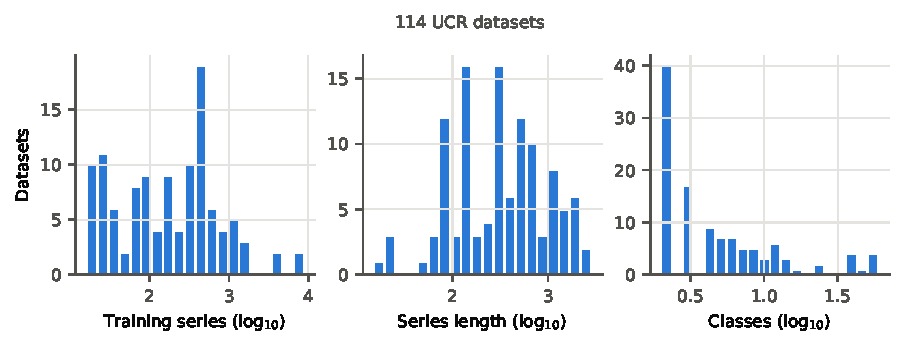
\includegraphics[width=\textwidth]{fig_datasets.pdf}
\caption{Training-set size, series length and number of classes of the \NDatasets{} UCR datasets.}\label{fig:datasets}
\end{figure}

\begin{figure}[h]
\centering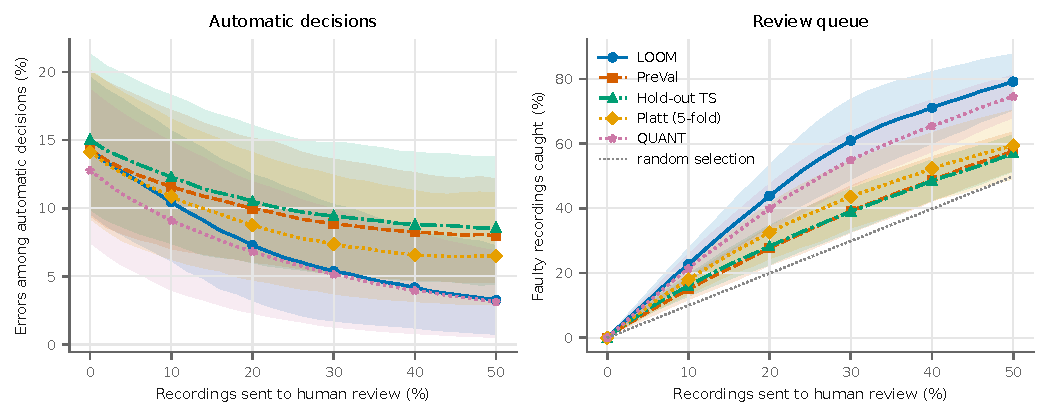
\includegraphics[width=\textwidth]{fig_triage_exploratory.pdf}
\caption{Exploratory triage study (12 datasets), same layout as Fig.~\ref{M-fig:triage} of the main text.}\label{fig:triagex}
\end{figure}

\begin{figure}[h]
\centering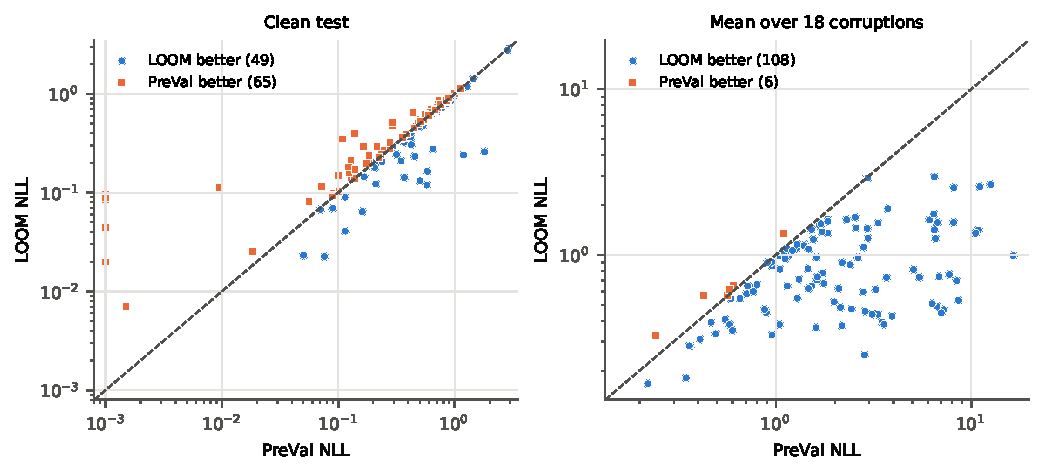
\includegraphics[width=\textwidth]{fig_scatter_loom_vs_preval.pdf}
\caption{Per-dataset NLL of LOOM against PreVal on clean data (left) and averaged over 18 simulated faults (right); points below the diagonal favour LOOM; values below $10^{-3}$ are drawn at $10^{-3}$.}\label{fig:scatter}
\end{figure}

\begin{figure}[h]
\centering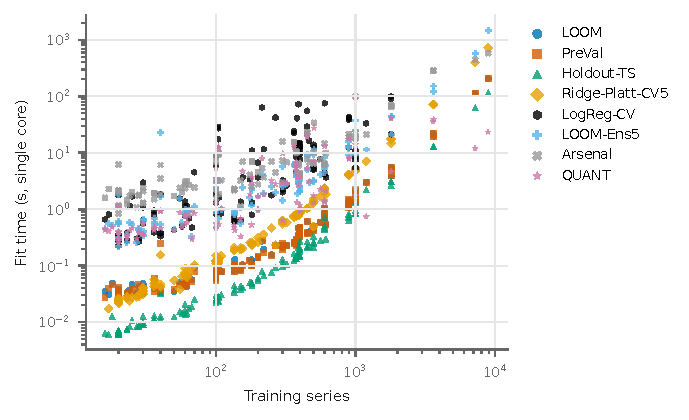
\includegraphics[width=0.7\textwidth]{fig_efficiency.pdf}
\caption{Fit time against the number of training series (log--log, single core).}\label{fig:eff}
\end{figure}

\bibliography{references}

\end{document}
